\documentclass[12pt, a4paper]{article}
\usepackage[utf8]{inputenc}
\usepackage[croatian]{babel}
\usepackage[margin=1in]{geometry}
\usepackage{amsmath}
\usepackage{amssymb}
\usepackage{amsthm} 
\usepackage{mathtools}
\usepackage{hyperref}
\usepackage{graphicx}
\usepackage{multirow}
\usepackage{fancyhdr} % prored, numeriranje stranice...
\usepackage{amsfonts}
\usepackage{setspace}% za postavljanje praznina
\usepackage{color}
\usepackage{wasysym}
\usepackage{bbm}
\usepackage{lscape}
\usepackage{filecontents}
\usepackage{multicol}
\usepackage{url}
\DeclareMathOperator {\sg}{sg}
\fancyhf{}
\renewcommand{\headrulewidth}{0pt}
\rfoot{\thepage}
\usepackage{paralist}
\usepackage{color}
\usepackage{tikz}
\usetikzlibrary{arrows,positioning,automata}
\PassOptionsToPackage{usenames,dvipsnames,svgnames}{xcolor}
 \newcommand{\HRule}{\rule{\linewidth}{0.5mm}}
\setlength\parindent{24pt}
\DeclarePairedDelimiter\floor{\lfloor}{\rfloor}
\DeclarePairedDelimiter\ceil{\lceil}{\rceil}
\usepackage{listings}
\usepackage{xcolor}


\begin{document}
\begin{multicols}{3}
\noindent 
\scriptsize
\textbf{Opće stvari:\\}
\textbf{Zbrajanje točaka} na eliptičkoj krivulji: \[E \, : \; y^2=x^3+ax+b\] Neka je $P=(x_1, x_2), Q=(y_1,y_2)$ onda je:
\[-\mathcal{O}=\mathcal{O}\]
\[-P=(x_1,-y_1)\]
\[\mathcal{O} + P=P\]
\[P+(-P)=\mathcal{O}\]
Za $Q \neq -P$, onda je $P+Q=(x_3,y_3)$ gdje je:
\[x_3=\lambda ^2-x_1-x_2\]\[y_3=-y_1+\lambda (x_1-x_3)\]
\[\lambda=\begin{cases}\frac{y_2-y_1}{x_2-x_1} &\mbox{ if } x_2 \neq x_1 \\ \frac{3x_1^2+a}{2y_1} &\mbox{ if } x_2=x_1 \end{cases}\]
\textbf{Formula za računanje reda grupe} $E(\mathbb{F}_p)$ gdje je $E: y^2=x^3+ax+b$:
\[|E(\mathbb{F}_p)|=p+1+\]\[\sum_{x \in F_p} \left(\frac{x^3+ax+b}{p}\right)\]
\textbf{Legendreov simbol:} $\left(\frac{x^3+ax+b}{p}\right)$ se računa prema:\\
Neka je $p$ neparan prost broj, $\left(\frac{a}{p}\right)$ je jednak 1 ako je $a$ kvadratni ostatak modulo $p$, -1 ako je $a$ kvadratni neostatak modulo $p$, a $0$ ako $p|a$.\\
Prema Eulerovom kriteriju vrijedi:
\[\left(\frac{a}{p}\right)\equiv a^{\frac{p-1}{2}} \textrm{ (mod } p)\]
Ako kongruencija $x^2\equiv a \textrm{ (mod }m) $ ima rješenja, kažemo da je $a$ \textbf{kvadratni ostatak} modulo $m$, u protivnom kažemo da je $a$ kvadratni neostatak modulo $m$.\\
Kažemo da je $a$ \textbf{kvadratno slobodan} ako je $1$ najveći kvadrat koji dijei $a$.\\[0.5cm]
\textbf{Prva DZ:} 1) Neka je $E \, : \; y^2=x^3+ax+b$ eliptička krivulja kojoj trebamo odrediti sve proste brojeve u kojima ima lošu redukciju te njen minimalni model. Najprije izračunamo diskriminantu te rastavimo ju na proste faktore: 
\begin{align}
\label{eq: diskrim}
\Delta&=-16(4a^3+27b^2)\\
&=p_0^{\alpha_0}...p_k^{\alpha_k}
\end{align}
$E$ ima dobru redukciju svugdje osim u $p_0,...,p_k$, ta se redukcija da popraviti ako postoji $j \in \{0,..,k\}$ takvi da $12|\alpha_j$. Ukoliko ne postoji takav $j$ loša redukcija se neće moći ukloniti, ipak ako postoji $l$ td $\alpha_l \geq 12$ i $p_l\neq 2,3$ možemo doći do minimalnog modela $E' \, : \; y'^2=x'^3+a'x'+b'$ uvodeći supstituciju: $x=p_l ^2x'$ i $y=p_l ^3 y'$. \textbf{Za određivanje tipa redukcije} tražimo $x_1, x_2, x_3 \in {\mathbb{F}_p}_l$ takav da je 
{\footnotesize \[f(x)=x^3+a'x+b' \equiv 0 (\textrm{ mod } p_l)\]}
U slučaju da se radi o trostukom korijenu radi se o aditivnoj redukciji, inače je redukcija multiplikativna i jedan je korijen dvostruki ($x_1=x_2$ ili $x_2=x_3$). Zapišemo $f_1(x)=(x-x_1)^2(x-x_3)$ te $f_2(x)=(x-x_1)(x-x_3)^2$ i pogledamo koja se od $f_1$ ili $f_2$ poklapa $x \in {\mathbb{F}_p}_l$  sa $f$. Pretpostavimo da je to $f_1$, uvodi se supstitucija $x'=x''+x_1$ i $y'=y''$ te uvrstimo to u minimalan model 	iz čega dobivamo novu eliptičku krivulju $E'' : y^2(x)=g(x)$, a za pripadnu funkciju $g(x)$ vrijedi: $g(x)=x^2(x-x_3+x_1)$. Ako jednadžba $\alpha ^2=-x_3+x_1$ ima rješenje u ${\mathbb{F}_p}_l$ tangente u singularnoj točki $(x_1,0)$ imaju koeficijente smjera koji su riješenja jednadžbe  $\alpha ^2=-x_3+x_1$ pa govorimo o podijeljenoj multiplikativnoj redukciji u $p=p_l$, inaće govorimo o nepodijeljenoj multiplikativnoj redukciji.
\textbf{Dvije eliptičke krivulje su ekvivalnetne} nad algebarski zatvorenim  poljem akko im se $j$-invarijante poklapaju. $\mathbb{Q}$ nije algebarski zatvoreno pa je potrebno vidjeti je li za supstituciju $(x,y) \to (u^2x, u^3y)$ $u \in \mathbb{Q}$.
\\ Druga DZ: \textbf{Singularnost krivulje i supstitucije} $E':\, y^2+a_1xy+a_3y=x^3+a_2x^2+a_4x+a_6$. Uvode se supstitucije: $b_2=a_1^2+4a_2$, $b_4=a_1a_3+2a_4$, $b_6=a_3^2+4a_6$, $b_8=\frac{1}{4}(b_2b_6-b_4^2)$, $E': y^2=4x^3+b_2x^2+2b_4x+b_6$, zatim se dalje uvode supstitucije: $c_4=b_2^2-24b_4$ i $c_6=-b_2^3+36b_2b_4-216b_6$ te se dobiva krivulja: $E: y^2=x^3-27c_4x-54c_6$. Gledamo diskriminantu:\[\Delta=\frac{c_4^3-c_6^2}{1728}\]
Vrijedi: $\Delta=0 $ akko krivulja singularna.\\
\[f(x,y)=x^3+a_2x^2+a_4x+a_6\]\[-(y^2+a_1xy+a_3y)\]
Točka $(x_0, y_0)$ je singularna akko $\partial_x f(x_0,y_0)=\partial_y f(x_0,y_0)=0$. Provjeravamo je li $(x_0,y_0)$ zadovoljava jdbu krivulje, ako da uvodimo supstituciju $t=\frac{y-y_0}{x-x_0}$ , odnosno
\begin{equation}
\label{eq:supst}
y=t(x-x_0)+y_0 
\end{equation}
(nadajmo se da je $y_0=0$). Umjesto $y$ u $f(x,y)=0$ uvrstimo  $t(x-x_0)+y_0$. Iz te jednadžbe dobijemo sređivanjem izraza (gdje je $x^3$ mi stavimo $((x-x_0)+x_0)^3$) $x-x_0=g(t)$ i umjesto $x-x_0$ u \ref{eq:supst} ubacimo $g(t)$ i dobijemo $y=tg(t)+y_0$. Pa je racionalna parametrizacija krivulje dana sa $\phi (t)=(g(t), tg(t)+y_0)$ .
\end{multicols}
\begin{multicols}{3}
\noindent
\scriptsize
\textbf{Određivanje reda i generatora grupe $E(\mathbb{F}_p)$} gdje je $E : y^2=f(x)$. Pogledamo za koje $x_0 \in \mathbb{F}_p$ dana jdba ima rješenja i koja su to (za $y$ možemo dobiti više riješenja jer riješavamo $y^2\equiv \alpha \, (mod \, p)$) Označimo ih s $(x_1,y_1), (x_2, y_2),...,(x_l,y_l)$ gdje se može dogoditi $x_i=x_j$, za $i \neq j$. Red grupe $|E(\mathbb{F}_p|=|\{(x_1,y_1),...,(x_l,y_l), \mathcal{O}\}|=l+1$. Uzmemo neku točku $Q$ iz $E(\mathbb{F}_p)$, i pogledamo vrijedi li da je ta točka generator grupe, odnosno, vrijedi li da je $\forall P \in E(\mathbb{F}_p)$ postoji $l \in {1,...,l}$ takav da je \[[l]Q=\underbrace{Q+Q+...+Q}_l=P\]
\textbf{Traženje torzijske grupe $E(\mathbb{Q})_{tors}$}. Računamo $\Delta_0=4a^3 +27b^2 = p_0^{\alpha_0}...p_l^{\alpha_l}$. Sada za  proste brojeve $q \not\in \{p_0,...,p_l\}$ promatramo $|E(\mathbb{F}_q|$ (obično se gleda do prvog prostog broja većeg od $p_l$. Neka su to $q_0,...,q_k$. Promatramo \[nzd(\{E(\mathbb{F}_q) : q \in \{q_0,..., q_k\}\})\]. Pretpostavi se da je to red grupe (to služi kao svojevrsna provjera). $y^2| \Delta_0$ pa gledamo zapravo $p_j$ takve da  $\alpha_j \geq 2$. Promatramo polinome $f(x)=x^3+ax+b-y_0^2$ gdje 
\[y_0 \in \left\{d: d| \prod_{\begin{subarray}{l} j=0\\ \alpha_j \geq 2 \end{subarray}}^l p_j^{\alpha_j}\right\}\]
i gledamo postoje li njegove cjelobrojne nultočke. Neka je $y_0$ neki fiksan iz gornjeg skupa takav da je $x_0$ neka cjelobrojna nultočka polinoma $f(x)$. Tada je $P=(x_0, y_0)$ generator od $E(\mathbb{Q})_{tors}$, a red te grupe je $m \in \mathbb{N}$ takav da $[m]P=\mathcal{O}$, a $E(\mathbb{Q})_{tors}\cong \mathbb{Z}_m$ gdje je onda $m \in \{1,2,3,4,5,6,7,8,9,10,12\}$ ili   $E(\mathbb{Q})_{tors}\cong\mathbb{Z}_2 \times \mathbb{Z}_{\frac{m}{2}}$ gdje je onda $m \in \{4,8,12,16\}$.
\end{multicols}
\begin{multicols}{3}
\scriptsize
\noindent
\textbf{Opći oblik jednadžbi krivulja sa torzijskim grupama}:\\
$\mathbb{Z}_2 \times \mathbb{Z}_4$:
\[y^2=(x-\alpha)(x- \beta)(x-\gamma),\] \[\, \alpha,\beta,\gamma \in \mathbb{Q}\]
$\mathbb{Z}_2 \times \mathbb{Z}_4$:
\[y^2=x(x+r^2)(x+s^2), \, r,s \in \mathbb{Q}\]
Za $\mathbb{Z}_2 \times \mathbb{Z}_8$: 
\[y^2=x(x+r^2)(x+s^2), \, r,s \in \mathbb{Q}\]
gdje su $rs,r(r+s), s(r+s)$ kvadrati racionalnih brojeva.\\
$\mathbb{Z}_2 \times \mathbb{Z}_4$:
\[y^2=(x+r^2)(x+s^2)\left(x+\frac{r^2s^2}{(r-s)^2}\right),\]\[r,s \in \mathbb{Q}\]
\textbf{Rang krivulje} \[E: y^2=x^3+ax^2+bx\]
Uvjet nesingularnosti: $\Delta=16b^2(a^2-4b)\neq 0$. Njoj pripadna 2-izogena krivulja ima jednadžbu: \begin{align*}E': y^2&=x^3-2ax^2+(a^2-4b)x\\&=x^3+a'x^2+b'x
\end{align*}
Za računanje ranga krivulje $E$ promatramo odgovarajuća preslikavanja $\alpha$ i $\beta$ te određujemo $|Im(\alpha)|$ i $|Im(\beta)|$.
Za $|Im(\alpha)|$ tražimo $(M,e,N)$ takve da jdba:
\[b_1 M^4+aM^2e^2+b_2 e^4=N^2\]
ima riješenja gdje:
\begin{itemize}
\item $b_1$ djelitelj od $b$ koji je kvadratno slobodan
\item $b_1b_2=b$
\item $(M,e)=1$
\end{itemize}
Pripadne jednadžbe uvijek promatramo u parovima jer je jednadžba simetrična. Dakle riješenja za $(b_1,b_2)$ su simetrična riješenjima za $(b_2,b_1)$ (onda riješenje $(b_1,b_2)$ brojimo 2 puta, a ovo drugo uopće ne promatramo). Broj takvih $(M,e,N)$ gdje pripadna jednadžba ima riješenja je $|Im(\alpha)|$.  Analogan postupak je za $b_1', b_2'$ gdje vrijede isti uvjeti, a broj rješenja pripadnih jednadžbi je $|Im(\beta)|$. U konačnici vrijedi da je \[2^{rank(E)=\frac{|Im(\alpha)||Im(\beta)|}{4}}\]
\end{multicols}
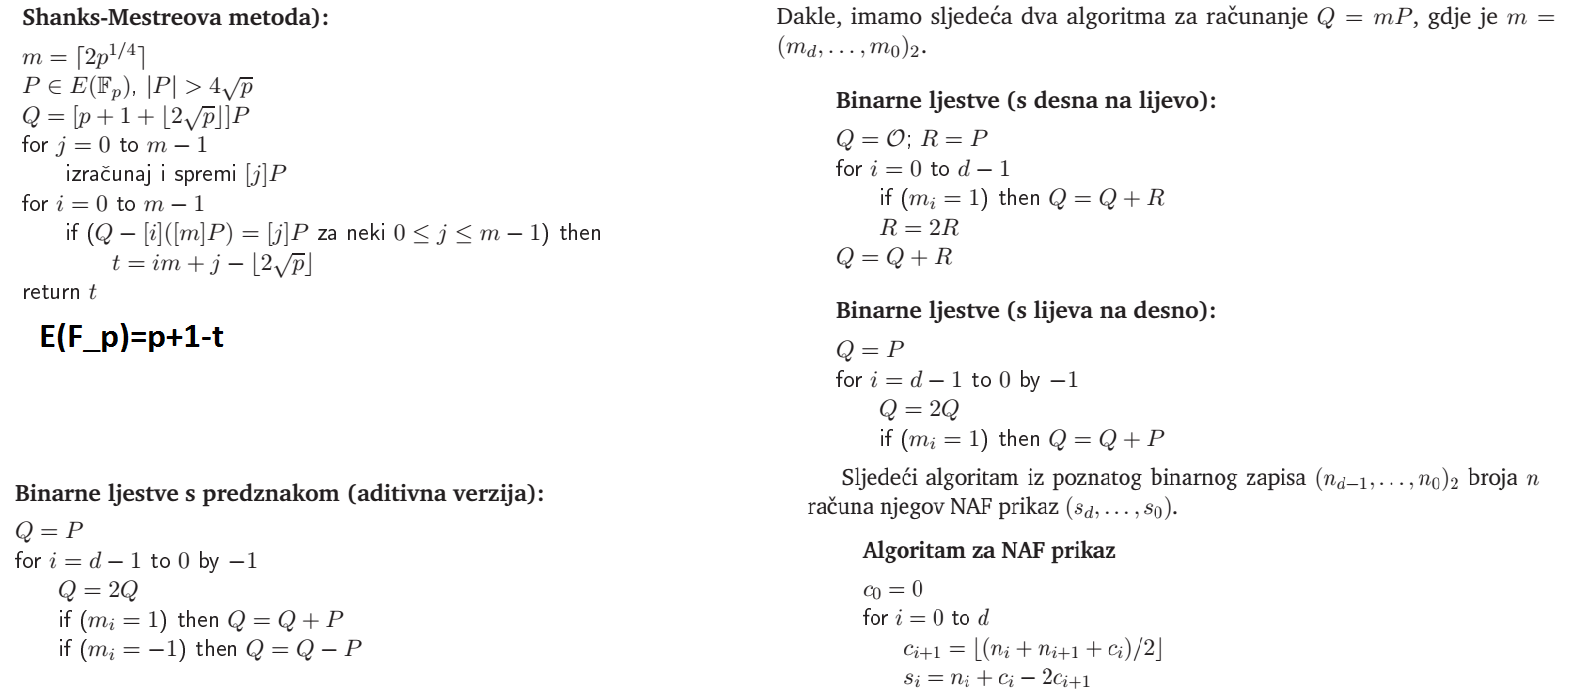
\includegraphics[scale=0.4]{algovi.png}
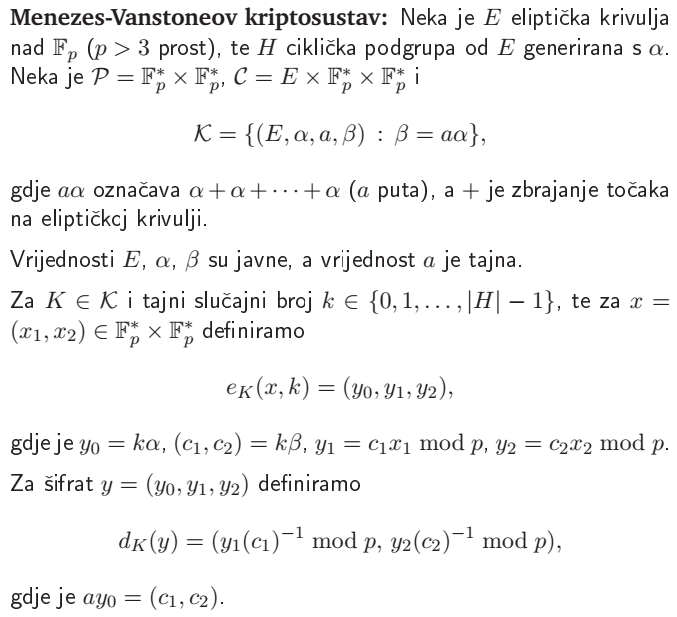
\includegraphics[scale=0.5]{mens.png}
\end{document}